\documentclass[11pt,a4paper]{article}

\usepackage[T1]{fontenc}
\usepackage[utf8]{inputenc}
\usepackage{lmodern}
\usepackage{microtype}
\usepackage[a4paper,margin=22mm,headheight=15pt]{geometry}
\usepackage{xcolor}
\usepackage{graphicx}
\usepackage{booktabs}
\usepackage{tabularx}
\usepackage{array}
\usepackage{enumitem}
\usepackage{listings}
\usepackage{fancyhdr}
\usepackage{hyperref}
\usepackage[most]{tcolorbox}

\definecolor{CassandraBlue}{HTML}{173752}
\definecolor{CassandraGreen}{HTML}{26734D}
\definecolor{CassandraGold}{HTML}{B7791F}
\definecolor{CassandraLight}{HTML}{EEF4F8}
\definecolor{CassandraGray}{HTML}{4B5563}
\definecolor{CodeBackground}{HTML}{F5F7F9}

\hypersetup{
  colorlinks=true,
  linkcolor=CassandraBlue,
  urlcolor=CassandraBlue,
  pdftitle={Cassandra R3v 1.0.0 User Manual},
  pdfauthor={Rosario Alia},
  pdfsubject={User manual for the public Cassandra R3v 1.0.0 release},
  pdfkeywords={Rul3volution, Cassandra, C-MAPSS, RUL, fuzzy systems}
}

\setlist[itemize]{leftmargin=*,itemsep=2pt,topsep=4pt}
\setlist[enumerate]{leftmargin=*,itemsep=3pt,topsep=4pt}
\setlength{\parindent}{0pt}
\setlength{\parskip}{5pt}
\renewcommand{\arraystretch}{1.15}

\lstdefinestyle{cassandra}{
  basicstyle=\ttfamily\small,
  backgroundcolor=\color{CodeBackground},
  frame=single,
  rulecolor=\color{CassandraBlue!25},
  breaklines=true,
  columns=fullflexible,
  keepspaces=true,
  showstringspaces=false,
  xleftmargin=4pt,
  xrightmargin=4pt,
  aboveskip=6pt,
  belowskip=6pt
}
\lstset{style=cassandra}

\newtcolorbox{importantbox}[1][]{
  enhanced,
  breakable,
  colback=CassandraLight,
  colframe=CassandraBlue,
  boxrule=0.8pt,
  arc=2pt,
  left=8pt,right=8pt,top=6pt,bottom=6pt,
  #1
}

\newtcolorbox{warningbox}[1][]{
  enhanced,
  breakable,
  colback=CassandraGold!8,
  colframe=CassandraGold,
  boxrule=0.8pt,
  arc=2pt,
  left=8pt,right=8pt,top=6pt,bottom=6pt,
  #1
}

\pagestyle{fancy}
\fancyhf{}
\fancyhead[L]{\small\textcolor{CassandraGray}{Cassandra R3v 1.0.0}}
\fancyhead[R]{\small\textcolor{CassandraGray}{User Manual}}
\fancyfoot[C]{\small\thepage}
\renewcommand{\headrulewidth}{0.4pt}
\renewcommand{\footrulewidth}{0pt}

\begin{document}
\pagenumbering{gobble}

\begin{titlepage}
  \pagecolor{CassandraLight}
  \color{CassandraBlue}
  \vspace*{18mm}

  {\Huge\bfseries CASSANDRA\par}
  \vspace{3mm}
  {\Large R3v 1.0.0\par}
  \vspace{10mm}
  {\huge\bfseries User Manual\par}
  \vspace{4mm}
  {\Large Interpretable prognostics with Rul3volution\par}

  \vspace{16mm}
  \begin{tcolorbox}[
    colback=white,
    colframe=CassandraBlue,
    boxrule=1pt,
    arc=3pt,
    left=10pt,right=10pt,top=10pt,bottom=10pt
  ]
    \color{black}
    This manual describes the public Cassandra R3v 1.0.0 release prepared for
    reproducible research use and future alignment with the associated scientific work. It covers installation, the desktop and
    command-line workflows, experiment artifacts, evaluation, diagnostics,
    and responsible interpretation of results.
  \end{tcolorbox}

  \vfill
  {\large\bfseries Rosario Alia\par}
  \vspace{2mm}
  {\large 20 September 2026\par}
  \vspace{7mm}
  {\normalsize GNU GPL v3 or later\par}
  \vspace{3mm}
  {\small Document version 1.0.0\par}
\end{titlepage}
\nopagecolor
\pagenumbering{roman}

\tableofcontents
\clearpage
\pagenumbering{arabic}

\section{Purpose and scope}

Cassandra R3v is the first public software implementation of the
Rul3volution method for Remaining Useful Life (RUL) estimation. Version 1.0.0
operates on the four NASA C-MAPSS turbofan subsets and implements a transparent
normalized zero-order Takagi-Sugeno model with readable fuzzy rules.

The software separates four quantities for every rule:

\begin{itemize}
  \item antecedent activation, denoted by $\mu_i$;
  \item consequent, denoted by $c_i$;
  \item positive global relative authority, denoted by $a_i$;
  \item normalized local responsibility, denoted by $\beta_i$.
\end{itemize}

AutoStructure can propose and validate new conjunctions built with \texttt{AND}.
Validation is performed on TRAIN engines only. Official TEST endpoints are used
after the structure is frozen.

\begin{importantbox}
\textbf{Release identity.} Scientific results attributed to Cassandra must be
generated from Git tag \texttt{v1.0.0}, with the commit identifier and experiment
profile recorded. This release is a public software reference for R3v and is intended to support
reproducibility and alignment with the associated article.
\end{importantbox}

\subsection{What this release demonstrates}

Version 1.0.0 demonstrates that the complete Rul3volution workflow is executable,
auditable, and reproducible on a realistic prognostics benchmark. It does not
claim state-of-the-art superiority over unrestricted black-box models, causal
explanations, or industrial deployment validation.

\section{Requirements and installation}

\subsection{System requirements}

\begin{itemize}
  \item Python 3.10 or newer;
  \item NumPy 1.24 or newer;
  \item pandas 2.0 or newer;
  \item Tkinter for the desktop interface;
  \item sufficient storage for NASA C-MAPSS and generated artifacts.
\end{itemize}

No GPU is required. Cassandra can run on x86-64 and ARM64 systems when compatible
Python packages are available.

On Debian, Ubuntu, or Linux Mint, install the system components with:

\begin{lstlisting}[language=bash]
sudo apt install python3 python3-venv python3-tk
\end{lstlisting}

\subsection{Install from the source release}

From the repository root:

\begin{lstlisting}[language=bash]
python3 -m venv .venv
source .venv/bin/activate
python -m pip install --upgrade pip
python -m pip install .
cassandra-r3v --version
\end{lstlisting}

The last command must report \texttt{cassandra-r3v 1.0.0}.

On Windows, use:

\begin{lstlisting}
py -3 -m venv .venv
.venv\Scripts\activate
python -m pip install .
\end{lstlisting}

\subsection{Start Cassandra}

From an unpacked source release:

\begin{lstlisting}[language=bash]
./run_cassandra.sh
\end{lstlisting}

Alternatives are:

\begin{lstlisting}[language=bash]
python3 run_cassandra.py
cassandra-r3v gui
\end{lstlisting}

On Windows, double-click \texttt{run\_cassandra.bat}. The desktop launchers print
the Cassandra banner before the window opens. Headless commands do not print the
banner.

\section{NASA data and the Cassandra workspace}

NASA C-MAPSS data are not included in the repository. Obtain the Turbofan Engine
Degradation Simulation data from an official NASA source under its applicable
terms. Cassandra accepts either the outer NASA archive or the inner
\texttt{CMAPSSData.zip} archive.

The release acceptance run used an archive with SHA-256:

\begin{lstlisting}
c9c5dec12a945a82e8bb4446589d7fb3cc057b5e5d81fa1a12e25ee9912ad3b2
\end{lstlisting}

This digest identifies the tested archive. Another archive may contain the same
NASA files but have a different digest because of repackaging.

Cassandra stores data and generated evidence in a separate workspace. The
default command-line workspace is \texttt{cassandra\_workspace}. Do not commit
this directory to the public repository.

\begin{warningbox}
\textbf{Data boundary.} Preparation, standardization, fuzzy partitions,
pseudo-endpoints, candidate screening, and structural validation use TRAIN only.
TEST data are reserved for final evaluation.
\end{warningbox}

\section{Desktop interface}

The top bar defines a shared scope. Select one or more subsets from FD001 to
FD004 and one or both protocols. The same selections apply to every stage.
Cassandra prevents an empty subset or protocol selection.

\begin{figure}[htbp]
  \centering
  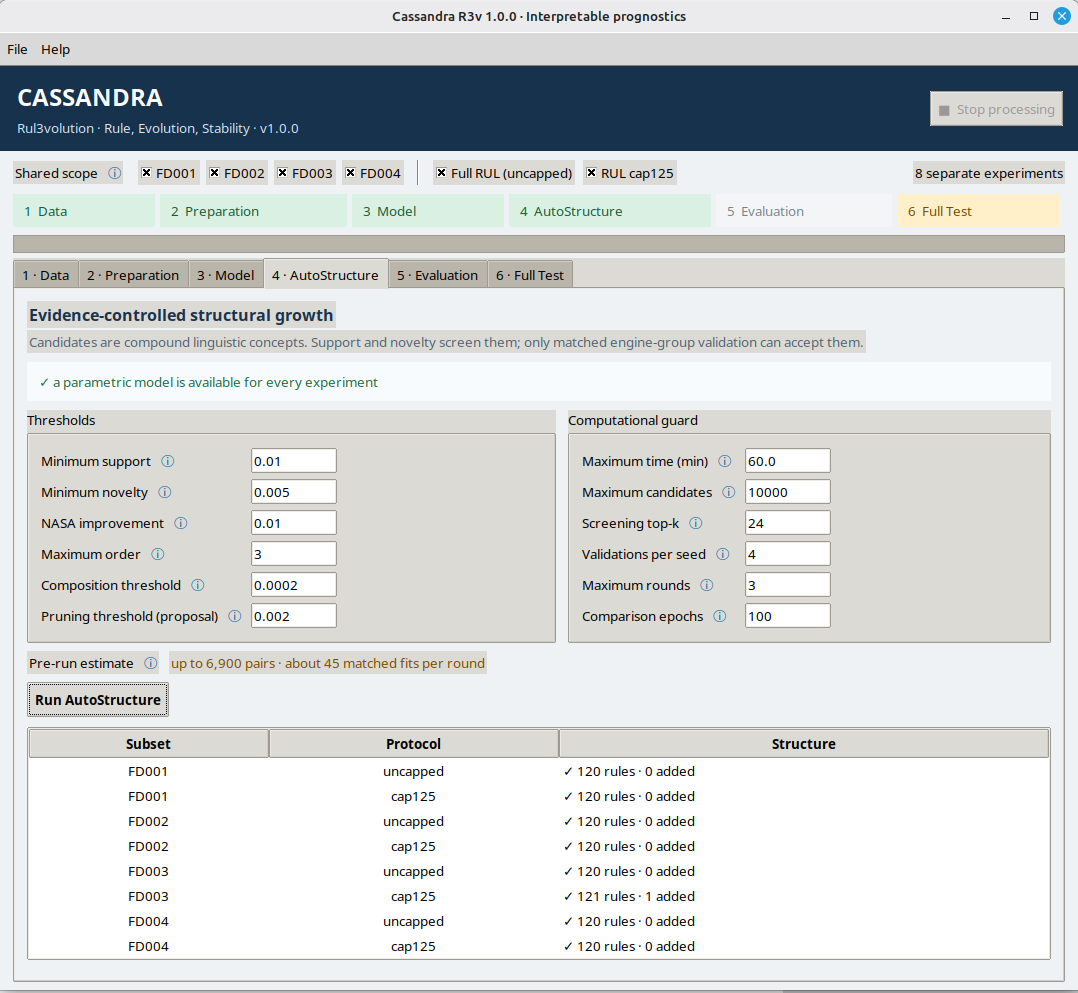
\includegraphics[width=0.96\textwidth]{assets/cassandra_gui_autostructure.png}
  \caption{The AutoStructure stage with all eight experiments selected. The
  table shows seven unchanged backbones and one accepted conjunction for
  FD003/cap125 in the canonical acceptance campaign.}
  \label{fig:gui}
\end{figure}

The workflow strip summarizes prerequisites:

\begin{itemize}
  \item \textcolor{CassandraGreen}{green}: all selected experiments are ready;
  \item yellow: only part of the selected scope is ready;
  \item light gray: a required stage is missing;
  \item blue gray: an optional stage is available;
  \item Full Test becomes green after a passing report.
\end{itemize}

Labels marked with an information symbol are clickable. They open a local
explanation beside the relevant control. During a calculation,
\textbf{Stop processing} requests cancellation at the next safe checkpoint. The
application remains open and incomplete temporary output is not accepted as a
valid artifact.

\section{End-to-end guided workflow}

Run the stages in order. Each subset/protocol pair is an independent experiment,
so selecting all four subsets and both protocols creates eight experiments.

\subsection{Stage 1: Data}

Choose the NASA archive and import it. Cassandra extracts and verifies the files
required for FD001--FD004. Importing does not create prepared experiments.

\textbf{Successful outcome:} the Data row for every available subset is ready.

\subsection{Stage 2: Preparation}

Run Preparation for the shared scope. Cassandra constructs leakage-safe
artifacts separately for \texttt{uncapped} and \texttt{cap125}.

\begin{itemize}
  \item \texttt{uncapped}: the target is the complete observed RUL range;
  \item \texttt{cap125}: the target is clipped at 125 cycles.
\end{itemize}

Standardization, fuzzy partitions, and pseudo-endpoints are fitted on TRAIN only.
The protocols must never be averaged or treated as interchangeable.

\textbf{Successful outcome:} one NPZ preparation exists for every selected pair.

\subsection{Stage 3: Model}

Run Model to train the 120-rule Full24 unary backbone. Cassandra uses five
linguistic levels for each of the 24 physical channels. Cycle and RUL are not
antecedent inputs.

Training writes:

\begin{itemize}
  \item \texttt{model\_backbone.json}: the retained frozen reference;
  \item \texttt{model.json}: the current model, initially identical to the backbone.
\end{itemize}

\textbf{Successful outcome:} both model files exist and the interface reports
120 rules for the initial structure.

\subsection{Stage 4: AutoStructure}

AutoStructure screens compound linguistic concepts and accepts a conjunction
only when support, novelty, matched engine-group validation, and seed consensus
satisfy the configured criteria. At most one rule is accepted per round.

The canonical settings include three validation seeds, a two-seed consensus,
a maximum order of 3, three rounds, and a 60-minute guard per experiment. The
pre-run estimate explains the maximum screening workload.

\begin{importantbox}
Returning \texttt{120 rules - 0 added} is a valid result. It means that no
candidate met the evidence requirements. AutoStructure is not required to add a
rule in every experiment.
\end{importantbox}

By default, a new AutoStructure run restarts from
\texttt{model\_backbone.json}. Use continuation from the current model only when
an explicitly continued structural search is intended.

The pruning threshold produces proposals only. Version 1.0.0 never deletes a
rule automatically and does not implement \texttt{OR} consolidation.

\subsection{Stage 5: Evaluation}

Evaluation applies the frozen backbone and the final model to the same official
TEST engines. It writes final-model metrics, local rule decompositions, and a
paired backbone--AutoStructure comparison.

Inspect the NASA score first: lower is better. Also inspect MAE, RMSE, $R^2$,
bias, individual engine penalties, and the uncertainty interval.

For a selected endpoint, the explanation table reports $\mu_i$, $a_i$,
$\beta_i$, $c_i$, and $\beta_i c_i$. The sum of rule contributions reconstructs
the prediction exactly. This is a faithful decomposition, not a causal claim.

\subsection{Stage 6: Full Test}

Full Test performs a non-destructive release and workspace audit. It checks the
runtime, source integrity, numerical contracts, source tests, raw data,
preparations, models, AutoStructure reports, evaluations, paired comparisons,
short pipeline paths, and a bounded structural-validation path.

A TXT report is saved automatically under \texttt{cassandra\_workspace/reports}.
Use \textbf{Save Report As...} to copy it elsewhere.

\begin{warningbox}
\textbf{Meaning of PASS.} A Full Test PASS proves that the calculation and
artifacts are valid. It does not prove that AutoStructure improved predictive
performance.
\end{warningbox}

\clearpage
\section{Worked example: FD003 with cap125}

This example illustrates how to read an AutoStructure outcome. Select only
\texttt{FD003} and \texttt{RUL cap125}, then run all six stages in order with the
canonical profile.

In the release acceptance campaign, AutoStructure accepted this conjunction:

\begin{importantbox}
\texttt{OS1\_Altitude IS LOW AND S20\_W31\_HPTCoolantBleed IS LOW}
\end{importantbox}

The structure grew from 120 to 121 rules. Official TEST evaluation produced:

\begin{center}
\begin{tabularx}{0.86\textwidth}{>{\bfseries}X r}
\toprule
Quantity & Value \\
\midrule
Backbone NASA score & 855.452 \\
Final NASA score & 823.922 \\
Point improvement & $+3.686\%$ \\
Paired 95\% bootstrap interval & $[-7.676\%,\ +9.488\%]$ \\
Conclusion & \texttt{inconclusive} \\
\bottomrule
\end{tabularx}
\end{center}

The correct interpretation is precise:

\begin{itemize}
  \item AutoStructure executed correctly and accepted one TRAIN-validated rule;
  \item the final TEST point estimate was better;
  \item the 95\% interval included zero;
  \item therefore, the TEST improvement was not statistically supported at the
  declared interval level.
\end{itemize}

Small floating-point differences can occur across platforms. Structural
decisions near a threshold must be checked against saved artifacts rather than
assumed to be bitwise identical.

\section{Interpreting the paired comparison}

The paired analysis resamples complete TEST engines 20,000 times with the fixed
seed \texttt{20260916}. Positive gain means that the final NASA score is lower.

\begin{tabularx}{\textwidth}{>{\ttfamily}p{0.28\textwidth} X}
\toprule
\normalfont\bfseries Conclusion & \bfseries Meaning \\
\midrule
no\_change & Backbone and final endpoint predictions are identical. \\
supported\_improvement & The complete 95\% gain interval is above zero. \\
supported\_degradation & The complete 95\% gain interval is below zero. \\
inconclusive & The interval includes zero. The point estimate alone is not
enough to claim improvement or degradation. \\
\bottomrule
\end{tabularx}

TEST results never accept, reject, or tune a rule. Their purpose is final
measurement after TRAIN-only structural selection.

\section{Command-line workflow}

The desktop and command-line interfaces use the same implementation and artifact
contract. The complete canonical sequence is:

\begin{lstlisting}[language=bash]
cassandra-r3v --workspace cassandra_workspace \
  import-data /path/to/nasa_cmapss.zip

cassandra-r3v --workspace cassandra_workspace prepare \
  --subsets FD001 FD002 FD003 FD004 \
  --protocols uncapped cap125

cassandra-r3v --workspace cassandra_workspace train \
  --subsets FD001 FD002 FD003 FD004 \
  --protocols uncapped cap125 \
  --epochs 250 --learning-rate 0.025 \
  --ridge 0.9 --patience 50

cassandra-r3v --workspace cassandra_workspace autostructure \
  --subsets FD001 FD002 FD003 FD004 \
  --protocols uncapped cap125 \
  --min-support 0.01 \
  --activation-support-cutoff 0.01 \
  --min-novelty 0.005 \
  --min-relative-improvement 0.01 \
  --folds 3 --seeds 7 42 99 \
  --consensus-required 2 --max-order 3 \
  --screen-top-k 24 \
  --pruning-threshold 0.002 \
  --parent-threshold 0.0002 \
  --validation-epochs 100 --max-minutes 60 \
  --max-candidates 10000 \
  --validations-per-seed 4 --max-rounds 3

cassandra-r3v --workspace cassandra_workspace evaluate \
  --subsets FD001 FD002 FD003 FD004 \
  --protocols uncapped cap125

cassandra-r3v --workspace cassandra_workspace full-test \
  --subsets FD001 FD002 FD003 FD004 \
  --protocols uncapped cap125
\end{lstlisting}

The exact scientific profile is stored in
\texttt{examples/article\_profile.json}. If an experiment changes these values,
the replacement profile and complete command line must be disclosed.

\clearpage
\section{Artifacts and evidence}

\begin{lstlisting}
cassandra_workspace/
|-- raw/extracted/
|-- prepared/FDxxx/{uncapped,cap125}.npz
|-- models/FDxxx/{uncapped,cap125}/
|   |-- model_backbone.json
|   `-- model.json
|-- structures/FDxxx/{uncapped,cap125}/autostructure.json
|-- evaluations/FDxxx/
|   |-- {uncapped,cap125}.json
|   `-- {uncapped,cap125}_backbone_vs_autostructure.json
|-- reports/cassandra_full_test_<timestamp>.txt
`-- archive/<timestamp>/
\end{lstlisting}

\begin{tabularx}{\textwidth}{>{\ttfamily\footnotesize}p{0.39\textwidth} X}
\toprule
\normalfont\bfseries Artifact & \bfseries Purpose \\
\midrule
prepared/*.npz & TRAIN-fitted arrays, targets, partitions, and metadata. \\
model\_backbone.json & Frozen 120-rule reference model. \\
model.json & Current final model after any accepted growth. \\
autostructure.json & Candidate screening, validation, consensus, and accepted rules. \\
evaluation JSON & Final TEST metrics and faithful local decompositions. \\
*\_backbone\_vs\_autostructure.json & Paired TEST effect and bootstrap uncertainty. \\
Full Test TXT & Software and artifact acceptance evidence. \\
\bottomrule
\end{tabularx}

Before using a number in an article, preserve the tag, commit SHA, environment,
machine description, command line, data hashes, experiment profile, generated
artifacts, and Full Test report. Article tables must come from evaluation JSON,
not from smoke-test metrics.

\section{Troubleshooting}

\subsection*{The GUI does not open}

Confirm that Tkinter is installed and that a graphical session is available:

\begin{lstlisting}[language=bash]
python3 -c "import tkinter; print(tkinter.TkVersion)"
\end{lstlisting}

On a headless server, use the command-line workflow.

\subsection*{A stage is disabled}

Read the dependency strip and the message at the top of the tab. Complete the
earliest missing prerequisite. For example, Model requires Preparation, and
Evaluation requires a model.

\subsection*{AutoStructure adds no rules}

This is not an error. Open \texttt{autostructure.json} or inspect the GUI status
to determine whether candidates failed support, novelty, validation, consensus,
or a computational guard.

\subsection*{AutoStructure takes too long}

Run experiments separately. Screening top-k, candidate, validation, time, and
round limits bound the workload. Changing canonical values creates a new
experimental profile and must be reported.

\subsection*{Full Test reports SKIP}

Missing NASA data or scientific artifacts may be skipped because they are not
distributed with the source. A present but invalid artifact is not treated as a
skip. For release acceptance, import the data, generate all eight experiments,
and rerun Full Test.

\subsection*{A previous artifact becomes outdated}

Cassandra archives dependent downstream artifacts when an upstream stage is
recomputed. Regenerate the affected stages instead of mixing files from
different runs.

\section{Scientific limitations and responsible use}

Version 1.0.0 has explicit boundaries:

\begin{itemize}
  \item fuzzy partitions remain fixed after TRAIN fitting;
  \item instantaneous inputs are used without age or temporal gradients;
  \item candidate generation can be expensive despite filters and hard guards;
  \item local decompositions are faithful but not causal;
  \item pruning proposals do not remove rules automatically;
  \item disjunctive \texttt{OR} consolidation is not implemented;
  \item one paired TEST set can leave a structural effect inconclusive;
  \item no claim of industrial deployment or universal predictive superiority is made.
\end{itemize}

These limitations do not invalidate Cassandra as an implementation. They define
the claims that can be supported by the current release and identify directions
for later research.

\section{Further documentation and citation}

The repository includes:

\begin{itemize}
  \item \texttt{README.md}: immediate overview and quick start;
  \item \texttt{docs/GUI\_GUIDE.md}: detailed interface behavior;
  \item \texttt{docs/REPRODUCIBILITY.md}: canonical scientific campaign;
  \item \texttt{docs/METHOD\_ALIGNMENT.md}: method-to-code contract;
  \item \texttt{docs/VALIDATION\_REPORT.md}: release evidence;
  \item \texttt{docs/PUBLISHING.md}: GitHub publication checklist;
  \item \texttt{CITATION.cff}: machine-readable citation metadata.
\end{itemize}

\clearpage
\thispagestyle{empty}
\pagecolor{CassandraLight}
\vspace*{\fill}

\begin{center}
{\LARGE\bfseries\textcolor{CassandraBlue}{Using and citing Cassandra}}\\[4mm]
\end{center}

If Cassandra is used in scientific work, cite the tagged software release and
the associated article. After archival, use the DOI displayed on the release
page. The software is distributed under GNU GPL v3 or later.

\begin{importantbox}[colback=white]
\textbf{Recommended reporting sentence.} ``Cassandra R3v 1.0.0 provides a
reproducible first implementation and feasibility demonstration of the
Rul3volution workflow on NASA C-MAPSS. Predictive effects of structural growth
are reported with paired uncertainty and are not generalized beyond the
available evidence.''
\end{importantbox}

\vfill
\begin{center}
\textcolor{CassandraGray}{\small End of Cassandra R3v 1.0.0 User Manual}
\end{center}
\nopagecolor

\end{document}
